\documentclass[dvipdfmx,12pt]{beamer}

\usepackage{bxdpx-beamer}
\usepackage{pxjahyper}
\usepackage{minijs}
\usetheme{AnnArbor}
\usepackage{mathpazo}
\usepackage{amsmath,amssymb}
\usepackage{graphicx}
\usepackage{array}
\usepackage{tikz}
\usepackage{wrapfig}
\usepackage{float}
\usepackage{here}
\usepackage{lscape}
\setbeamertemplate{navigation symbols}{}

\title{Reference Dependence and Monetary Incentive}
\subtitle{-Evidence from Major League Baseball-}
\author{Reio TANJI}
\date{Dec 14th, 2018}
\institute{Osaka University}

\begin{document}

\begin{frame}\frametitle{}
\titlepage
\end{frame}

\section{Introduction}

\begin{frame}\frametitle{Abstract}
  \begin{itemize}

    \item Using the data of Major League Baseball (MLB), we analyzed the relationship between observed reference dependent behavior and monetary incentives.

    \item MLB players evaluate their performance indexes as an outcome, with the reference dependent preference.

    \item They adjust their effort levels in order to achieve the reference points of the performance indexes, even though there are NOT observed any monetary incentives.
  \end{itemize}
\end{frame}

\section*{Table of Contents}
\begin{frame}\frametitle{Contents}
  \tableofcontents
\end{frame}

\section{Literature and Contribution}
\begin{frame}\frametitle{Reference Dependence}
  \begin{itemize}
    \item Individuals evaluate outcomes by the relative value to their internal benchmarks, or reference point, not by their absolute ones: reference dependence

    \item Reference dependence enabled us to interpret some inconsistent empirical decision making with the traditional microeconomic theory, by applying additional assumptions.

    \item There are a lot of following researches that shows the evidence for the reference dependence in field and laboratory settings, including about athletes' decision making.

    : Performance of sports is measured by nonmonetary outcomes.

  \end{itemize}
\end{frame}

\begin{frame}\frametitle{Literature}
  \begin{itemize}

    \item Pope and Schweizer (2011) pointed out that for the professional golf players regard ``par'' as the reference point, which results in the different probability of success in their putts.

    \item Allen et al. (2016) specified the existance of reference point dependence of marathon runners, using data about the finish time of enormous number of race in the United States.

    $\Rightarrow$ Runners try to goal before the round numbers, and it results in observed excess mass, or ``bunching'' around 4 hours.

  \end{itemize}

\end{frame}

\begin{frame}\frametitle{Literature}
  \small
  Pope and Simonsohn (2011)
  \begin{tabular}{lr}
    \begin{minipage}[H]{0.45\textwidth}
      \footnotesize
      \begin{itemize}
        \item picked up the case of Major League Baseball (MLB) players, about the observed attitude to their performance indexes.

        \item MLB position players manipulate their batting-average (AVG), in order to meet their internal goals: .300

        \item As a result, there is observed excess mass, or ``bunching'' around .300 of AVG.
      \end{itemize}

    \end{minipage} &
    \begin{minipage}[H]{0.55\textwidth}
      \begin{figure}
        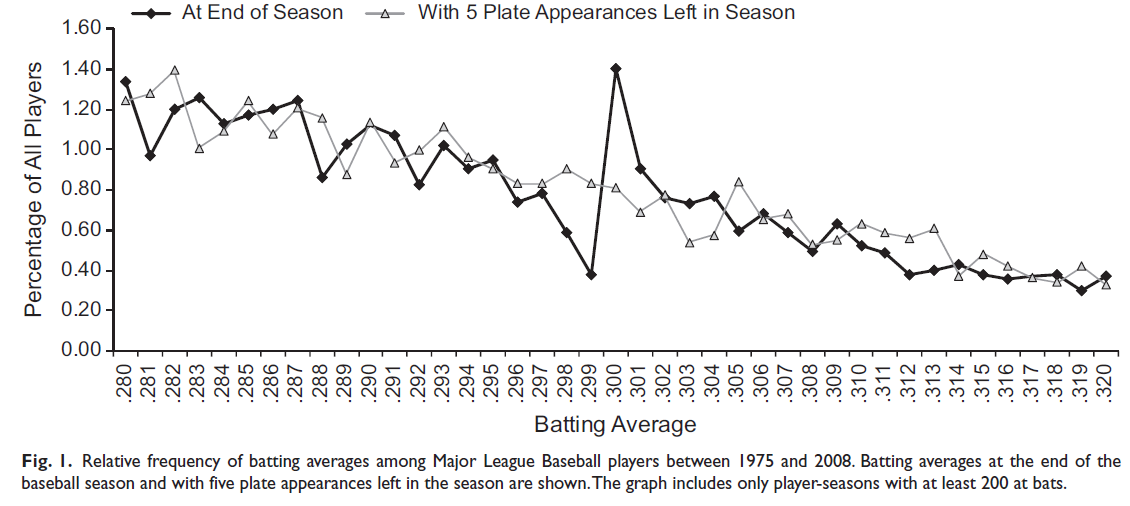
\includegraphics[keepaspectratio, scale = 0.33]{graphs/PS_fig1}
        \caption{Excess Mass Around .300 (quated from Pope and Simonsohn (2011))}
        \label{PS_fig}
      \end{figure}
    \end{minipage}
  \end{tabular}

\end{frame}

\begin{frame}\frametitle{Extention and Contribution}
\begin{itemize}
  \item The case of MLB is different from that of marathon, in that players receive monetary rewards according to the contracts they signed.

  \item Their contracts might include some incentivesed parts, which pay them additional bonus when their AVG reaches a certain cutoff point.

  \item The contribution of our research is to examine this: examine if there exists any monetary incentives that make players make effort to the cutoff point.
\end{itemize}
\end{frame}

\section{Frameworks and Empirical Methods}
\begin{frame}\frametitle{Theoretical Frameworks}
  \begin{tabular}{lrr}
    \begin{minipage}[H]{0.4\textwidth}
      \begin{figure}[H]
        \begin{tikzpicture}[domain = 0:4, samples = 200, >= stealth]
          \draw[->](-0.5, 0) -- (4.2, 0) node[right]{$x$};
          \draw[->](0, -0.5) -- (0, 3.7) node[above]{$u(x)$};
          \draw[-](2.2, -0.1) -- (2.2, 0.1);
          \draw[domain=0:2.2,samples=200,>=stealth] plot (\x, {sqrt(\x)});
          \draw[domain=2.2:4.1,samples=200,>=stealth] plot (\x, {sqrt(\x) + 0.8});
          \draw (0, 0) node[below left]{O};
          \draw (2.2, -0.3) node {$r$};
        \end{tikzpicture}
        \scriptsize
        \caption{discontinuous utility function}
        \label{jump}
      \end{figure}
      \end{minipage} &
      \begin{minipage}[H]{0.5\textwidth}
        \footnotesize
        \begin{itemize}
          \item Following Allen et al. (2016) assume utility function $u(x)$ that jumps at the cutoff point, or the reference point.

          $x$ stands for the performance index.

          \item This disconituity generates excess mass, or ``bunching'' around the possible reference point.

          \item We consider the possibility that this type of utility is derived by the discontinuous design of the monetary reward of the players.

        \end{itemize}
      \end{minipage}
  \end{tabular}

\end{frame}

\begin{frame}\frametitle{Flow of Specification}
  \begin{enumerate}
    \item First, confirm that there exists manipulation in AVG, including other round-numbers such as .200 or .350:

    Also, we examine this about other performance indexes.

    -- On-base percentage (OBP), homerun (HR), runs-batted-in (RBI), stolen-bases (SB), base-hit (H), and stolen-base (SB).

    \item Second, for the possible reference points, test if there are any monetary incentives: discontinuous design of the contracts.
  \end{enumerate}
\end{frame}

\begin{frame}\frametitle{Specification: Manipulation}

  \begin{tabular}{lr}
    \begin{minipage}[H]{0.45\textwidth}
      \small
      \begin{itemize}
        \item We exploit the McCrary (2007)'s manipulation test, which is used in regression discontinuity design.

        \item Make local approximation of the histgram of the variable of interest, and calculate the predicted values of $f(r)$ at the cutoff point, from both above and below there.
      \end{itemize}
    \end{minipage}
    &
    \begin{minipage}[H]{0.5\textwidth}
      \begin{figure}
        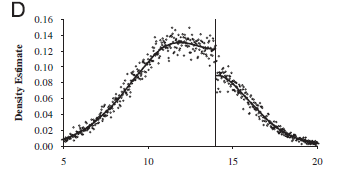
\includegraphics[keepaspectratio, scale = 0.8]{graphs/McCrary_figD.png}
        \caption{Discontinuous frequency (quated from McCrary(2007))}
        \label{McC}
      \end{figure}
    \end{minipage}
  \end{tabular}

\end{frame}

\begin{frame}\frametitle{Specification: Contract Design}
  \begin{itemize}
    \small
    \item Discontinuity of the contract design is tested by RDD methodology:

    \begin{align*}
      w_{it} = & \beta_0 X_{it} + \beta_1 \text{ABOVE}_{it} \\
      \text{where} \\
      w_{it}: & \text{ log salary of the next season} \\
      X_{it}: & \text{ performance index} \\
      \text{ABOVE}_{it}: & \text{ indicator for achievement}
    \end{align*}

    We also conduct analysis including other performance and other player specific charactaristics.

    \item To check the robustness of our results, we also conduct the same local regression including the interaction term of $X_{it}$ and $\text{ABOVE}_{it}$.

    \[
    w_{it} = \beta_0 X_{it} + \beta_1 \text{ABOVE}_{it} + \beta_2 X_{it} \times \text{ABOVE}_{it}
    \]

  \end{itemize}
\end{frame}

\begin{frame}\frametitle{Data}
  We obtain information about the players' stats (indexes) and annual salary.
  \begin{itemize}
    \item Stats Data
    \begin{itemize}
      \item From \textit{fangraphs}

      \item Play stats from 1957 to 2018

      \item We restrict the sample to the players with at least 200 plate-appearances $N=18143$
    \end{itemize}
    \item Salary Data
    \begin{itemize}
      \item From \textit{USA TODAY} and \textit{Baseball References}

      \item Contract information from 1987 to 2017 $N=8915$
      \begin{itemize}
        \item Fixed part of the salary of each player

        \item possession of free agency, the right to negotiate any team in MLB.
      \end{itemize}
    \end{itemize}
  \end{itemize}
\end{frame}

\section{Results}
\begin{frame}\frametitle{Results: Manipulation}
  \begin{figure}
    \centering
    \caption{Histgram of Batting-Average}        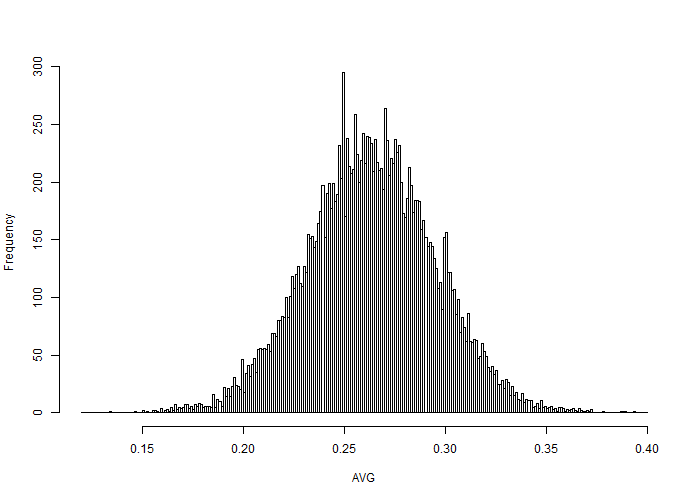
\includegraphics[keepaspectratio, scale = 0.35, angle=0]{graphs/hist_AVG_all.png}
    \label{AVG_Histgram}
  \end{figure}

\end{frame}

\begin{frame}
  \begin{figure}
    \centering
    \caption{Discontinuity at .300 of AVG}
    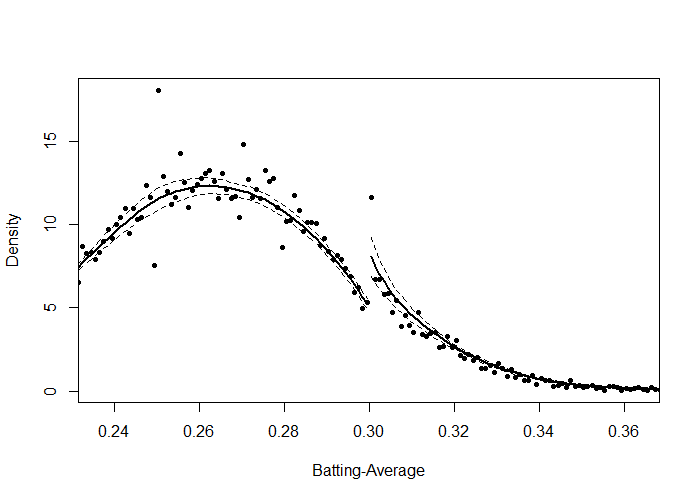
\includegraphics[keepaspectratio, scale = 0.5, angle = 0]{graphs/AVG_300.png}
    \label{DCdensity_AVG_300}

  \end{figure}
\end{frame}

\begin{frame}
  \begin{table}
    \tiny
    \centering
    \caption{Test for Manipulation, leastPA $= 200$}
    \begin{tabular}{lcccccc}\hline
      index & type & cutpoint & binsize & bandwidth & $\theta$ & $z$
      \\ \hline \hline
      AVG & rate & .300 & .001 & .019 &  .499 & 7.442*** \\
      & & & & & (.067) & \\
      & & .250 & .001 & .024 & .212 & 5.061*** \\
      & & & & & (.042) & \\
      OBP & rate & .350 & .001 & .024 &  .139 & 2.854** \\
      & & & & & (.049) &  \\
      HR & cumulative & 20 & 1 & 5.309 & .259 & 3.465*** \\
      & & & & & (.075)  & \\
      RBI & cumulative & 100 & 4 & 15.423 & .311 & 3.295*** \\
      & & & & & (.094) & \\
      SB & cumulative & 30 & 1 & 10.000 & .529 & 4.274*** \\
      & & & & & (.124) & \\
      & & 40 & 1 & 11.505 & .481 & 2.764** \\
      & & & & & (.174) & \\
      PA & cumulative & 500 & 1 & .003 & .160 & 2.515* \\
      & & & & &(.063) & \\
      H & cumulative & 200 & 1 & 18.922 & .453 & 2.547 * \\
      & & & & & (.178) & \\ \hline \hline
      Note & \multicolumn{6}{r}{
      ***: $p<0.1\%$, **: $p<1\%$, *: $p<5\%$.
      }\\
      \multicolumn{7}{r}{
      Bandwidth is optimized following the method of McCrary(2008).
      }
    \end{tabular}
    \label{Bunch-True}
  \end{table}
\end{frame}

\begin{frame}\frametitle{Results: Manipulation}
  \begin{itemize}
    \item In .300 of batting-average, there in fact exists manipulation by the players.

    \item Also in .250 of AVG and some of other round numbers of indexes, there were observed discontinuity:

    $\Rightarrow$Players consider these numbers as referene points and adjust their aspiration levels.

    \item Manipulation is not observed in all the round numbers.

  \end{itemize}
\end{frame}

\begin{frame}\frametitle{}
  \begin{table}[!]
    \caption{RDD Test for Monetary Incentives}
    \label{RDD_A}
    \tiny
    \centering
    \begin{tabular}{lccccccc}\hline
      index,cutpoint & Other Control & bw type & bandwidth
      & Observations & Estimate & Std. Error & $z$
      \\ \hline \hline
      AVG, .300 & No &LATE & .084 & 8514 & .047 & .061 & .773 \\
      & &Half-BW &  .042 & 5599 & .088 & .075 & 1.174 \\
      & & Double-BW & .170 & 8915  & .067 & .056 & 1.184 \\ \cline{3-8}

      & Yes &LATE & .045 & 5930 & .034 & .056 & .615 \\
      & &Half-BW &  .023 & 3005 & .061 & .077 & .788 \\
      & & Double-BW & .090 & 8605  & .016 & .045 & .354 \\ \hline

      AVG, .250 & No &LATE & .036 & 6110 & .019 & .068 & .286 \\
      & &Half-BW &  .018 & 3496 & .015 & .092 & .161 \\
      & & Double-BW & .072 & 8539  & .034 & .054 & .636 \\ \cline{3-8}

      & Yes &LATE & .048 & 7271 & .070 & .052 & 1.340 \\
      & &Half-BW &  .024 & 4402 & .066 & .069 & .953 \\
      & & Double-BW & .096 & 8810  & .075 & .044 & 1.713 \\ \hline

      HR, 20 & No & LATE & 3.32 & 1315 & .071 & .175 & .406 \\
      & & Half-BW & 1.66 & 562 & .073 & .127 & .576 \\
      & & Double-BW & 6.64 & 2582 & -.004 & .109 & -.034 \\ \cline{3-8}

      & Yes & LATE & 3.30 & 1307 & -.002 & .141 & -.015\\
      & & Half-BW &1.65 & 560 & .030 & .102 & .299 \\
      & & Double-BW & 6.61 & 2558 & -.032 & .088 & -.364 \\ \hline

      OBP, .350 & No &LATE & .044 & 6440 & -.038 & .065 & -.592 \\
      & & Half-BW & .021 & 3542 & -.076 & .089 & -.849 \\
      & & Double-BW & .087 & 8656 & -.029 & .051 & -.570 \\ \cline{3-8}

      & Yes & LATE & .045 & 6525 & -.013 & .049 & -.272 \\
      & & Half-BW & .022 & 3673 & -.055 & .069 & -.807 \\
      & &Double-BW & .089 & 8637 & .004 & .039 & .107 \\ \hline

      Note: & \multicolumn{7}{r}{***: $p<0.1\%$, **: $p<1\%$, *: $p<5\%$.} \\
      & \multicolumn{7}{r}{Bandwidth is optimized following the method of Imbens and Kalyanaraman (2009).} \\
      & \multicolumn{7}{r}{``Half'' and ``Double'' stands for using a half and twice of bandiwidths, respectively.} \\
      \multicolumn{8}{r}{
      ``Yes'' in ``Other Control'' shows including players' age (quadratic), FLD, BsR, FA dummy, Season and Position dummies.
      }
    \end{tabular}
  \end{table}
\end{frame}

\begin{frame}\frametitle{}
  
% Table created by stargazer v.5.2.2 by Marek Hlavac, Harvard University. E-mail: hlavac at fas.harvard.edu
% Date and time: ��, 12 04, 2018 - 13:49:29
\begin{table}[H] \centering
  \caption{Regression on Log-Salary, Including Interaction Term: around .300}
  \label{AVG300_A}
\fontsize{4pt}{4pt}\selectfont
\begin{tabular}{@{\extracolsep{-10pt}}lcccccc}
\\[-1.8ex]\hline
\hline \\[-1.8ex]
 & \multicolumn{6}{c}{\textit{Dependent variable:}} \\
\cline{2-7}
\\[-1.8ex] & \multicolumn{6}{c}{Loggarithm of Salary} \\
\\[-1.8ex] & \multicolumn{5}{c}{\textit{OLS}} & \textit{felm} \\
\\[-1.8ex] & (1) & (2) & (3) & (4) & (5) & (6)\\
\hline \\[-1.8ex]
 Constant & 11.166$^{***}$ & $-$6.616$^{***}$ & $-$5.203$^{***}$ & $-$5.319$^{***}$ & $-$5.319$^{***}$ &  \\
  & (.423) & (.665) & (.671) & (.667) & (.667) &  \\
  & & & & & & \\
 AVG & 11.513$^{***}$ & 11.620$^{***}$ & 4.361$^{***}$ & 4.221$^{***}$ & 4.221$^{***}$ & 3.808$^{**}$ \\
  & (1.537) & (1.209) & (1.209) & (1.201) & (1.201) & (1.189) \\
  & & & & & & \\
 AVG\_300 & $-$.169 & $-$.413 & $-$.191 & $-$.142 & $-$.142 & $-$.069 \\
  & (1.050) & (.821) & (.785) & (.780) & (.780) & (.706) \\
  & & & & & & \\
 FLD &  & .006$^{***}$ & .008$^{***}$ & .007$^{***}$ & .007$^{***}$ & .008$^{***}$ \\
  &  & (.002) & (.002) & (.002) & (.002) & (.002) \\
  & & & & & & \\
 BsR &  & .009$^{*}$ & .002 & .003 & .003 & .020$^{***}$ \\
  &  & (.005) & (.005) & (.005) & (.005) & (.005) \\
  & & & & & & \\
 AVG$\times$AVG\_300 & .663 & 1.428 & .681 & .540 & .540 & .160 \\
  & (3.429) & (2.681) & (2.566) & (2.549) & (2.549) & (2.312) \\
  & & & & & & \\
\hline \\[-1.8ex]
WPA &  &  & X & X & X & X \\
AGE (quadratic) &  & X & X & X & X &  \\
FA dummy &  &  & X & X & X &  \\
Season dummies &  & X & X & X & X & X \\
Position dummies &  &  & X & X & X &  \\
Fixed effects &  &  &  &  &  & Individual \\
Observations & 5,960 & 5,930 & 5,930 & 5,930 & 5,930 & 5,930 \\
R$^{2}$ & .035 & .420 & .470 & .478 & .478 & .744 \\
Adjusted R$^{2}$ & .035 & .416 & .466 & .473 & .473 & .660 \\
Residual Std. Error & 1.286 (df = 5956) & 1.001 (df = 5892) & .957 (df = 5881) & .950 (df = 5880) & .950 (df = 5880) & .764 (df = 4459) \\
F Statistic & 71.983$^{***}$ (df = 3; 5956) & 115.152$^{***}$ (df = 37; 5892) & 108.865$^{***}$ (df = 48; 5881) & 109.753$^{***}$ (df = 49; 5880) & 109.753$^{***}$ (df = 49; 5880) &  \\
\hline
\hline \\[-1.8ex]
\textit{Note:}  & \multicolumn{6}{r}{$^{*}$p$<$0.05; $^{**}$p$<$0.01; $^{***}$p$<$0.001} \\
& \multicolumn{6}{r}{The bandwidth is same as RDD for .300 of AVG.} \\
& \multicolumn{6}{r}{FLD and BsR stands for the contribution of the player to the team, expressed by the runs they earned.} \\
& \multicolumn{6}{r}{WPA is ``win-percentage added.''} \\
\end{tabular}
\end{table}

\end{frame}

\begin{frame}\frametitle{}
  \begin{table}[!]
    \caption{RDD Test for Monetary Incentives (Cont')}
    \label{RDD_A}
    \tiny
    \centering
    \begin{tabular}{lccccccc}\hline
      index,cutpoint & Other Control & bw type & bandwidth
      & Observations & Estimate & Std. Error & $z$
      \\ \hline \hline
      RBI, 100 & No & LATE & 4.08 & 393 & .072 & .289 & .250 \\
      & &Half-BW & 2.04 & 228 & .282 & .400 & .707 \\
      & &Double-BW & 8.16 & 714 & .008 & .185 & .043 \\ \cline{3-8}

      & Yes & LATE & 4.04 & 390 & .018 & .209 & .086 \\
      & & Half-BW & 2.02 & 227 & -.042 & .324 & .130 \\
      & & Double-BW & 8.07 & 708 & .056 & .127 & .435 \\ \hline

      H, 200& No & LATE & 3.173 & 75 & -.786 & .396 & -1.985* \\
      & & Half-BW & 1.587 & 35 & .386 & .271 & -1.421 \\
      & & Double-BW & 6.347 & 137 & -.061 & .309 & -.199 \\ \cline{3-8}

      & Yes & LATE & 3.175 & 75 & -.420 & 1.042 & -.403 \\
      & & Half-BW & 1.587 & 35 & -4.779 & .576 & -8.288** \\
      & & Double-BW & 6.349 & 137 & -.109 & .413 & -.265 \\ \hline

      SB, 30 & No & LATE & 3.39 & 282 & .962 & .372 & 2.585** \\
      & &Half-BW & 1.70 & 134 & .920 & .263 & 3.492*** \\
      & &Double-BW & 8.16 & 714 & .008 & .185 & 2.941** \\ \cline{3-8}

      & Yes & LATE & 3.40 & 282 & .379 & .297 & 1.271 \\
      & & Half-BW & 1.70 & 134 & .290 & .249 & 1.163 \\
      & & Double-BW & 6.79 & 533 & .408 & .180 & 2.260* \\ \hline

      SB, 40 & No & LATE & 3.16 & 134 & -1.276 & .453 & -2.818** \\
      & &Half-BW & 1.58 & 56 & -.736 & .383 & -1.924 \\
      & &Double-BW & 6.32 & 245 & -.712 & .313 & -2.274* \\ \cline{3-8}

      & Yes & LATE & 3.16 & 134 & -.346 & .396 & -.875 \\
      & & Half-BW & 1.58 & 56 & -.313 & .429 & -.730 \\
      & & Double-BW & 6.33 & 245 & -.115 & .244 & -.472 \\ \hline

      Note: & \multicolumn{7}{r}{***: $p<0.1\%$, **: $p<1\%$, *: $p<5\%$.} \\
      & \multicolumn{7}{r}{Bandwidth is optimized following the method of Imbens and Kalyanaraman (2009).} \\
      & \multicolumn{7}{r}{``Half'' and ``Double'' stands for using a half and twice of bandiwidths, respectively.} \\
      \multicolumn{8}{r}{
      ``Yes'' in ``Other Control'' shows including players' age (quadratic), FLD, BsR, FA dummy, Season and Position dummies.
      }
    \end{tabular}
  \end{table}
\end{frame}


\begin{frame}\frametitle{Results: Monetary Incentives}
  \begin{itemize}
    \item As a whole, there are not observed clear evidence for additional bonuses achieving some these round numbers.

    $\Rightarrow$ Players manipulate their performance indexes, even though there are little or no monetary incentives to do so.

    \item For 30 stolen-bases, our analysis does not show determinant results, so we should further results.

    \item Restricting the sample to the players with the right of free agency yields essentially the same results.

  \end{itemize}
\end{frame}

\begin{frame}\frametitle{Extention}
  \begin{itemize}
    \item By-Time analysis
    \begin{itemize}
      \item Replicate the same examination, but now we devide the sample by histrical terms:
      \begin{enumerate}
        \item Before the system of free agency regulated (-1975)

        \item Before the Strike of Players Association (-1994)

        \item Before \textit{Moneyball} (Lewis) was published (-2003)

        \item Afterward (2004-)

        * Note that because we obtain the sample of contract design only after '87, we cannot conduct the second analysis for before '86.
      \end{enumerate}

      \item Hakes and Sauer (2006) aregued that after the publication of \textit{Moneyball}, team managers regard on-base percentage as more important index to measure the players' contribution to the team they belong to.

    \end{itemize}
  \end{itemize}

\end{frame}

\begin{frame}
  \begin{table}
    \centering
    \caption{Manipulation Test for the Grouped Sample by Time}
    \label{Mani-Era}
    \tiny
    \begin{tabular}{lcccccc} \hline
      index, cutpoint &  & '57-'75 &'76-'94 & '95-2003 & 2004- &full sample \\ \hline \hline
      AVG, .300 & bw & .023 & .020 & .022 & .019 & .019 \\
      & $\theta$ & .573 & .566 & .310 & .403 & .499 \\
      & & (.146) & (.120) & (.130) & (.120) & (.067) \\
      & $z$ & 3.934*** & 4.732*** & 2.393* & 3.376*** & 7.442*** \\ \hline
      AVG, .250 & bw & .028 & .028 & .032 & .027 & .024 \\
      & $\theta$ & .250 & .151 & .306 & .121 & .212 \\
      & & (.080) & (.069) & (.094)& (.076) & (.042) \\
      & $z$ & 3.149** & 2.188* & 3.242** & 1.595 & 5.061*** \\ \hline
      OBP, .350 & bw & .031 & .030 & .036 & .030 & .024 \\
      & $\theta$ & .137 & .149 & -.035 & .137 & .139 \\
      & & (.089) & (.081) & (.093) & (.082) & (.049) \\
      & $z$ & 1.538 & 1.846 & -.380 & 1.672 & 2.854** \\ \hline
      HR, 20 & bw & 6.313 & 6.677 & 10.165 & 7.273 & 5.309 \\
      & $\theta$ & .222 & .214 & .145 & .315 & .259 \\
      & & (.150) & (.123) & (.129) & (.112) & (.075) \\
      & $z$ & 1.479 & 1.751 & 1.117 & 2.819** & 3.465*** \\ \hline
      Note & \multicolumn{6}{r}{
      ***: $p<0.1\%$, **: $p<1\%$, *: $p<5\%$.
      }\\
      & \multicolumn{6}{r}{
      Bandwidth is optimized following the method of McCrary(2008).
      }
    \end{tabular}
  \end{table}

\end{frame}

\begin{frame}
  \begin{table}
    \centering
    \caption{RDD for the Grouped Sample by Time}
    \label{RDD_Era}
    \tiny
    \begin{tabular}{lcccccc} \hline
      index, cutpoint & bw, type &  &'87-'94 & '95-2003 & 2004- &full sample \\ \hline \hline
      AVG, .300 & LATE & bw & .024 & .042 & .030 & .045 \\
      &  & Obs. & 697 & 1806 & 1872 & 5930 \\
      &  & estimate & -.034 & .064 & .066 & .034 \\
      &  & & (.137) & (.092) & (.103) & (.056) \\
      & & $z$ & -.250 & .697 & .637 & .615 \\ \hline
      AVG, .250 & LATE & bw & .036 & .043 &.075 & .048 \\
      &  & Obs. & 1482 & 1806 & 3991 & 7271 \\
      &  & estimate & .154 & .064 & .076 & .070 \\
      &  & & (.084) & (.092) & (.060) & (.052) \\
      & & $z$ & 1.825 & .697 & 1.277 & 1.340 \\ \hline
      HR, 20 & LATE & bw & 4.183 & 3.685 & 2.46 & 3.30 \\
      &  & Obs. & 341 & 371 & 475 & 1307 \\
      &  & estimate & -.255 & -.348 & .343 & -.002 \\
      &  & & (.228) & (.218) & (.264) & (.141) \\
      & & $z$ & -1.122 & -1.600 & 1.300 & -.015 \\ \hline
      OBP, .350 & LATE & bw & .031 & .025 & .027 & .045 \\
      &  & Obs. & 1098 & 1281 & 2042 & 6525 \\
      &  & estimate & .109 & -.151 & -.030 & -.013 \\
      &  & & (.106) & (.120) & (.093) & (.049) \\
      & & $z$ & 1.031 & -1.262 & -.323 & -.272 \\ \hline
      Note: & \multicolumn{6}{r}{***: $p<0.1\%$, **: $p<1\%$, *: $p<5\%$.} \\
      & \multicolumn{6}{r}{Bandwidth is optimized following the method of Imbens-Kalyanaraman.}
    \end{tabular}
  \end{table}
\end{frame}

\begin{frame}\frametitle{}
  \begin{itemize}
    \item About manipulation, players seems to be affected by the historical changes.

    \item However, .300 of batting-average has been a solid benchmarks for the players.

    \item On the other hand, team managers (since '87) does not propose any discontinuous form of contracts to the players.

    $\Rightarrow$ Again, we argure there does not exists no monetary incentive that leads them to manipulate indexes.

    \item Restricting the sample to the FA players also show the same.
  \end{itemize}
\end{frame}

\section{Conclusions}
\begin{frame}\frametitle{Conclusion}
  Main Findings
  \begin{enumerate}
    \item Players manipulate their performance indexes to meet them with some round numbers.

    \item There exist no monetary incentives in their contracts that makes players to do so.

    \item Tendency of the manipulation changes through the history of baseball.

    - Among them, especially, .300 of AVG shows consistent results, which shows it is solid benchmarks for the players.
  \end{enumerate}

  Note that some indexes require following research, obatining information that makes limitation of our analysis.
\end{frame}

\section*{Reference and Sources}

\begin{frame}\frametitle{Reference}
  \tiny
  \begin{thebibliography}{99}
    \bibitem PPope and Simonsohn. 2011.
    Round Numbers as Goals: Evidence From Baseball, SAT Takers, and the Lab
    \textit{Psychological Science} 22(1) 7179

    \bibitem HHakes and Sauer. 2006.
    An Economic Evaluation of the Moneyball Hypothesis
    \textit{Journal of Economic Perspectives} Volume 20, Number 3 - Summer 2006 - Pages 173185

    \bibitem AAllen, Dechow, Pope and Wu. 2016.
    Reference-Dependent Preferences: Evidence from Marathon Runners \textit{Management Science} 63(6):1657-1672.

    \bibitem PPope and Schweizer. 2011.
    Is Tiger Woods Loss Averse? Persistent Bias in the Face of Experience, Competition, and High Stakes
    \textit{American Economic Review} 101 (February 2011): 129157

    \bibitem{}Kahneman and Tversky. 1979.
    Prospect Theory: An Analysis of Decision under Risk.
    \textit{Econometrica}
    Journal of the Econometric Society47 (2):263291.

    \bibitem{}McCrary. 2007.
    Manipulation of the running variable in the regression discontinuity design: A density test
    \textit{Journal of Econometrics} 142 (2008) 698 - 714

    \bibitem{}Krautmann and Oppenheimer. 2002.
    Contract Length and the Return to Performance in Major League Baseball
    \textit{Journal of Sports Economics} February 2002

    \bibitem{}Tversky and Kahneman. 1992.
    Advances in Prospect Theory: Cumulative Representation of Uncertainty
    \textit{Journal of Risk and Uncertainty}, 5:297 - 323 (1992)

    \bibitem{}Imbens and Kalyanaraman. 2009.
    \textit{NBER Working Paper Series.} 14726

    \bibitem{}Alex Rees-Jones. 2018.
    Quantifying Loss-Averse Tax Manipulation
    \textit{Review of Economic Studies} (2018) 85, 1251 - 1278
  \end{thebibliography}

\end{frame}

\begin{frame}\frametitle{Data References}
  \begin{itemize}
    \item \textit{fangraphs Baseball}

    https://www.fangraphs.com/

    \item \textit{Baseball Reference}

    https://www.baseball-reference.com

    \item \textit{USA TODAY}

    https://www.usatoday.com/sports/mlb/

    \item \textit{Baseball Prospectus: Cot's Baseball Contracts}

    https://www.baseballprospectus.com/
  \end{itemize}
\end{frame}

\section*{Appendix}
\begin{frame}\frametitle{Contract Length}
  \begin{itemize}
    \item Krautmann and Oppenheimer (2002) pointed out that the longer the contract duration extend, the lower return to their performance is obtained: Players show the risk-aversion.

    \begin{align*}
      \ln(SAL_{it}) = \beta_1 &+ \beta_2 PERF_{it} \\
      &+ \beta_3 (PERF_{it} * LENGTH_{it})+ \beta_4 LENGTH_{it}
    \end{align*}
    \footnotesize
    \flushright
    * The model is quoted from Krautmann and Oppenheimer (2006).

    \flushleft
    \normalsize

    \item Estimated value of $\beta_3$ was negative.

    \item Further research considering the contract length to be required.
  \end{itemize}

\end{frame}


\begin{frame}\frametitle{Incentivised Contracts}
    \begin{itemize}
      \footnotesize
      \item Ichiro Suzuki, Outfielder, 4-year contract with Seattle Marinars (2004-'07)
      \begin{itemize}
        \footnotesize
        \item signing bonus- \$6M

        \item fixed payment- 04:\$5M, 05:\$11M, 06:\$11M, 07:\$11M

        \item performance bonuses- \$1.25M in performance bonuses for plate appearances

        \begin{itemize}
          \footnotesize
          \item \$50,000 each for 400 PAs, 2004-06

          \item \$0.1M each for 500 \& 600 PAs, 2004-06

          \item \$0.1M for 400 PAs, 2007

          \item \$0.2M each for 500 \& 600 PAs, 2007
        \end{itemize}

        \item award bonuses: \$50,000 each for Gold Glove, All Star selection

        \item trade-Protection (Veto for moving the team without his acceptance):

        limited no-trade clause (may block deals to 10 clubs)

        \item Other

        \begin{itemize}
          \footnotesize
          \item housing allowance: \$28,000 in 2004, \$29,000 in 2005, \$30,000 in 2006, \$31,000 in 2007

          \item interpreter, trainer, transportation for spring \& regular season

          \item 4 annual round-trip airline tickets from Seattle to Japan
        \end{itemize}
      \end{itemize}
    \end{itemize}
\end{frame}

\begin{frame}\frametitle{Incentivised Contracts}
  \begin{itemize}
    \footnotesize
    \item Eric Sogard, 2nd-baseman, single-year contract with Milwaukee Brewers (2018)
    \begin{itemize}
      \footnotesize
      \item fixed Payment- \$2.4M

      \item performance bonuses- : \$0.15M each for 30, 50, 70, 90 games. \$50,000 for 120 games
    \end{itemize}
  \end{itemize}

  \begin{itemize}
    \footnotesize
    \item Alex Avila, Catcher, two-year contract with Arizona Diamondbacks (2018, 2019)

    \begin{itemize}
      \footnotesize
      \item Fixed Payment- 18:\$4M, 19:\$4.25M

      \item annual performance bonuses: \$25,000 each for 350, 400 plate appearances. \$50,000 each for 450, 500 PA. \$0.1M for 550 PA.
    \end{itemize}
  \end{itemize}
\end{frame}

\begin{frame}
  \begin{itemize}
    \item We obtained details of the contracts about the active players in 2018 season from \textit{Cot's}.

    \item Players receive additional performance-dependent rewards:

    Award bonus and index-dependent bonus.

    \item Few position players sign the contract with index-dependent bonus, and all of them are related to the number of attendance:

    Plate-appearances, games-attended
  \end{itemize}
\end{frame}

\end{document}
